\chapter{集合论}

\section{集合的属性}
最基本的集合就是一组对象构成的集合,首先需要认识的是子集与全集.对于多个子集,可以定义交($\cap$)、并($\cup$)、补($\Sigma-A$).

单个最直接的属性就是集合的大小,这就是Cardinality.对于有限可数的集合,可以直接数出来有多少个元素,但对于无限集,需要通过映射的方式定义.

\subsection{基数、Card与映射}
对于两个无限集,假如存在一一对应,就说两个集合的Card( cardinality,基数)是相等的:$|A|=|X|$.通过这种方式可以证明有理数与整数一样多.比如$(0,1]$间的有理数可以按以下方式列出:
\begin{enumerate}
\item 分母为1的既约分数:1。
\item 分母为2的既约分数:$\frac{1}{2}$。
\item 分母为3的既约分数:$\frac{1}{3},\frac{2}{3}$。
\item 分母为$n$的既约分数,其个数小于$n-1$。
\end{enumerate}

对于基数,有以下论断:
\begin{enumerate}
\item 任意可列(可数)的无限集与自然数集等势,也有一说:与自然数等势的集合,被定义为可数无限集。
\item 自然数集的基数是$\aleph_0$,是最小的可列无限集。实数集的基数是$2^{\aleph_0}$。也就是说:自然数集的幂集与实数集等势。证明时可以考虑实数的二进制表达,构造两个单射:$\{0,1\}^N\rightarrow $与$[0,1)\rightarrow \{0,1\}^N$,有些实数有两种二进制表达,比如$(0.1)_{2}=(0.01111\cdots)_2$,所以约定不允许连续无限个1.
\item 无限集关于card的性质:设$X$是无限集,则
\begin{enumerate}
\item $|\mathbb{N}| \lesssim |X|$。意为$\mathbb{N}$是最小的无限基数。
\item $|X\times X|=|X|$。相当于说乘积空间与原空间等势。那么容易知道,$|\mathbb{N}\times \mathbb{N}|=|\mathbb{N}|$,这是因为前者是可列的:
\begin{center}
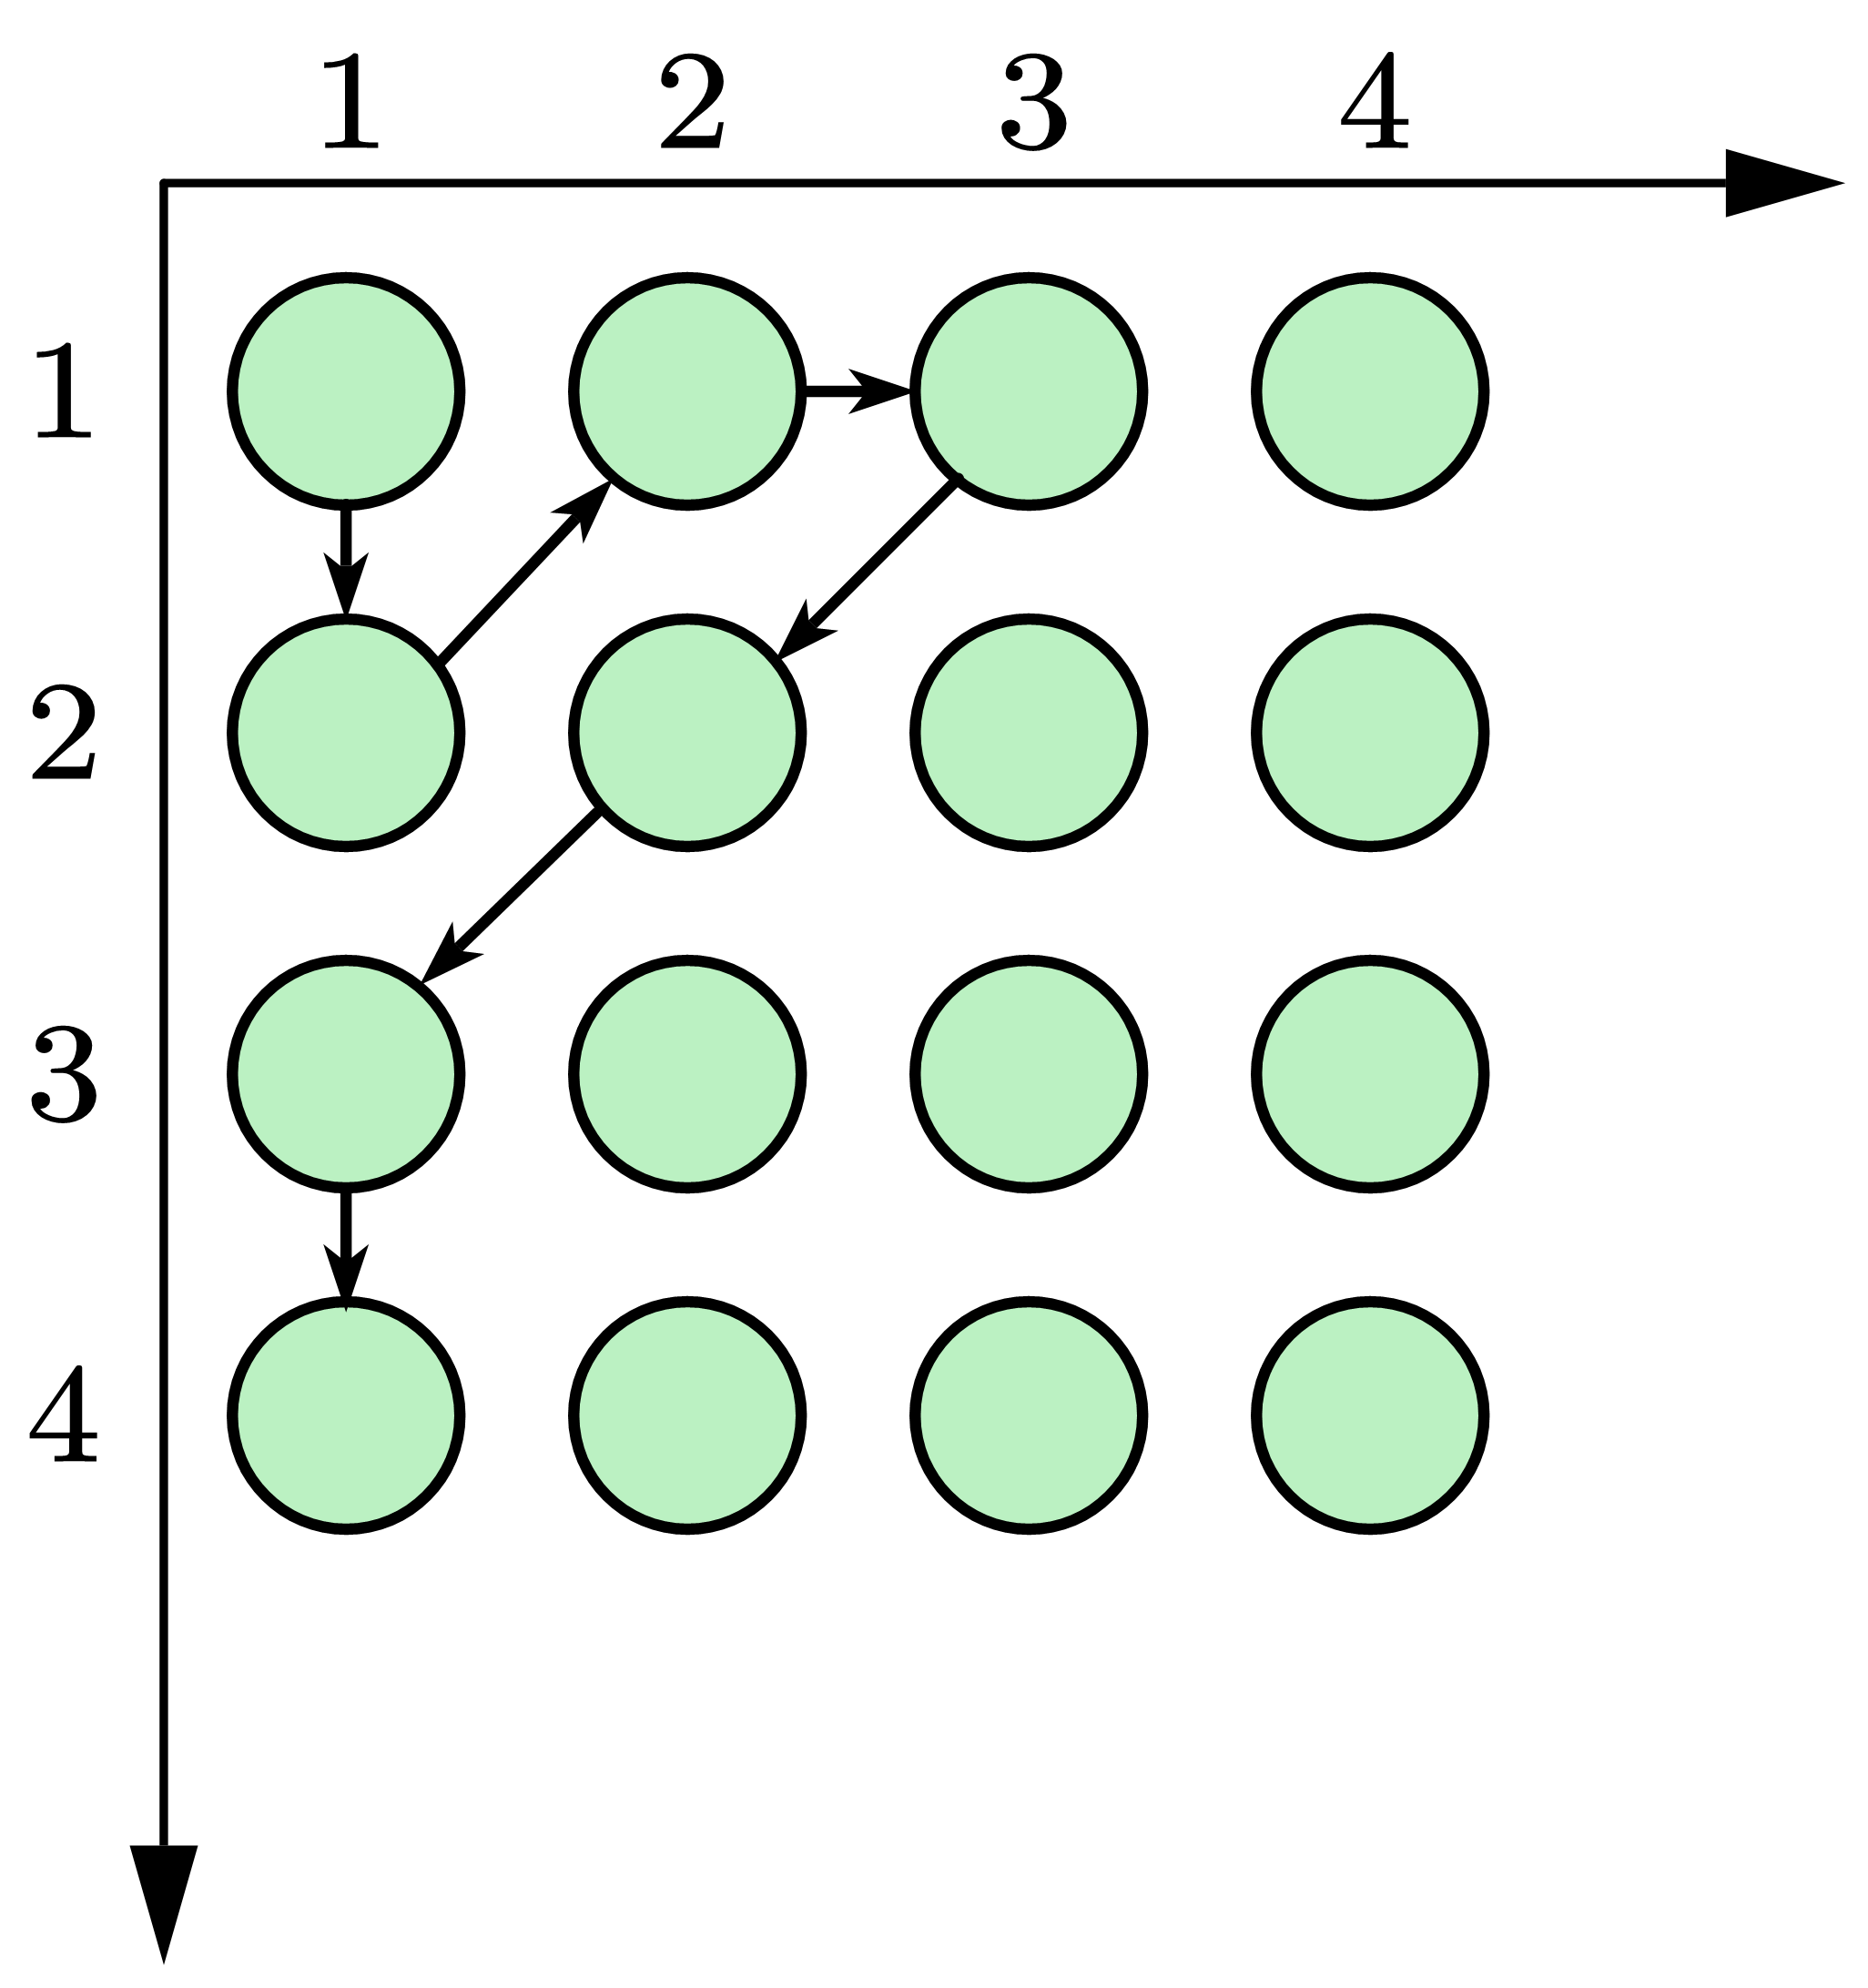
\includegraphics[width=5cm]{figure/2d-list.png}
\end{center}
同时,也有$|\mathbb{R}\times \mathbb{R}|=|\mathbb{R}|$,这是因为对于任意两个实数,可以按10进制展开,然后把它们的数字“交织”在一起形成一个实数。
\item $|\mathbb{R}|=|P(\mathbb{N})|$。$P(X)$为幂集。
\end{enumerate}
\item \emph{连续统假设}:任意实数的不可数子集,与整个实数集等势。这是希尔伯特的23个数学问题的第一个问题。它的另一表述是对基数进行排序:$\aleph_0,\aleph_1,\cdots$,那么$\aleph_{n+1}=2^{\aleph}$,则连续统假设断言:$\aleph_1=2^{\aleph_0}$。也可以说不存在$\aleph$,满足$\aleph_0<\aleph<2^{\aleph}$.

记$P(X)$为无限集合$X$的幂集,前者的基数是$2^{\aleph}$,后者为$\aleph$,\emph{广义连续统假设}认为:如果存在$A\subset P(X)$,且$A$与$P(X)$不等势,那么$|A|\leq |X|$。另一方面,这个假设是说,任意幂集的子集合,其基数不能大于$|X|$,所以广义连续统假设也可以表述为,对于任意无穷基数,不存在严格介于$\aleph$与$2^{\aleph}$之间的基数。哥德尔证明:连续统假设与ZFC是独立的,即假如ZF集合论没有矛盾,则连续统假设不能被ZFC证伪。
\end{enumerate}

仅仅有大小和一组对象还比较简单,给集合中的元素赋予相互关系,就可以构成更复杂的结构.比如给两个元素定义一个距离(距离空间、度量空间),那么就可以定义邻域($U(a)$)、开集、边界($\partial A$)、内部($\text{int} A$或者$\mathring{A}$)、闭包($\overline{A}$).

\subsection{测度}
测度是面积、长度概念的推广,直观上也相当于集合的大小,但基数描述大小主要是从计算的角度出发的,而测度主要是从积分的概念出发。首先要明确的是,测度是一个函数,将一个集合映射为实数,并且这个映射至少满足可加性。这就与范畴\ref{category}、同胚联系起来了。测度映射保持了可加性。以下列出一些比较重要的测度。

与分开密切相关的\emph{豪斯多夫测度(hausdorff)}:

\begin{empheq}{align*}
H^s_{\delta}(A)&=\inf\sbbra{2^{-s}\alpha(s)\sum_{j=1}^{\infty}|C_j|^s\middle| A\subset \bigcup_{j=1}^{\infty}C_j,|C_j|\leq \delta}\\
\alpha(s)&=\frac{\pi^{s/2}}{\Gamma(s/2+1)} \mtag{s维球面积}\\
H^s(A)&=\lim_{\delta\rightarrow 0} H^s_{\delta}(A) \mtag{s维Hausdorff Measure}
\end{empheq}

$|C_j|$为点集的直径,不要把它当成面积,比如对于一个直径为$\delta$的圆,那么$C_j\delta$。在$H^s_{\delta}(A)$的定义中,我们首先对区域进行拆分(为多个球),然后分别计算每个区域的测度,再线性组合起来。又定义\emph{豪斯多夫维数}为:
$$\dim_H(A)=\inf \sbbra{0\leq s<\infty \mid H^s(A)=C\neq 0<\infty}$$

由于计算维数时,仅仅要求测试为有限值,因此$\alpha(s)$和$\frac{1}{2^s}$的系数可以不要。这个维数的特点是,如果$s<\dim_H(A)$,那么有$H^s(A)=0$。$s$大于时,为无穷大。

豪斯多夫维数之所以与分形联系紧密,是因为它很好地描述了“倍增”。考虑二维边长为1的矩形,按边长$\delta$划分为小矩形,每个用圆来代替。那么忽略系数后,$h^s_{\delta}(A)=n^2|C_j|^s=\frac{1}{\delta^2}\delta^s$,要使这个值有限,显然$s=2$。另一个角度来看,一个正方形可以划分为4个小正方形,相当于说如果每条边缩小2倍,那么面积缩小4倍,即维数:
$$s=\frac{\ln 4}{\ln 2}=2$$

\paragraph*{零测集}零测集就是测度为0的集合,直到了十分关键的作用。

\begin{definition}[零测集]
对于集合$A\in\mathbb{R}^n$,如果$\forall \varepsilon>0,$,可以用可数个$n$维立方体覆盖$A$,且这些立方体的体积之和小于$\varepsilon$。则称$A$为零测集。形式化表述为:

$\forall \varepsilon>0,\exists U_n\in(a_n, b_n)^n$,满足$A\subset \cup U_n, \sum |U_n|<\varepsilon$。
\end{definition}

一个典型的例子是有理数集合,它是零测集。因为它是可列的:$\mathbb{Q}={q_1,q_2,\cdots}$,那么取覆盖$U_n=(q_n-3^{-n}\varepsilon,q_n+3^{-n}\varepsilon)$,这个覆盖的测度小于$\varepsilon$。

从以上例子也可以看出,可列集都是零测集。不过零测集不一定可列。
\subsection{邻域($U(a)$)}邻域是包含这个点的集合,并且稍微”抖动“一下也不会离开这个集合.常见的邻域如:

\begin{enumerate}
	\item 开球$U(x,\delta)$.
	\item 去心开球$U_0(x,\delta)$.
\end{enumerate}

\subsection{边界($\partial A$)}几种定义:

\begin{enumerate}
\item 边界=闭包-内部:
	$$\partial A=\overline{A}-\mathring{A}$$
\item 边界=闭包$\cap$补集的闭包:
	$$\partial A=\overline{A}\cap \overline{\Omega-A}$$
\item 边界是一系列点的集合,这些点的每一个领域都至少有一个点属于$A$,也至少有一个点不属于$A$:
	$$\partial A=\{x | \forall U(x), \exists p,q\in U(x), p\in A, q\notin A\}$$
	
	这种定义是最基本的定义.
\end{enumerate}

\subsection{内部($\mathring{A}$)}比较难理解.

\begin{enumerate}
	\item 内部就是非边界点.
	\item 内部是内点的集合,内点是指,存在以这些点为中心的邻域,包含于集合$A$中.
\end{enumerate}

单独一个圆${(x,y)|x^2+y^2=1}$是没有内部的,任取一个点,它的任意领域必然有点不属于这个圆.

假如一个集合内部为空,即$\mathring{A} \neq \emptyset$,相当于只有边界集.以二维平面来看,边界是线,我们在线上找不出一个圆形区域.因此内部为空,即$\nexists \text{非空开子集} O\in A$.反面就是,假如内部非空,则可以找到一个开子集$O$,它满足$O\in A, O\notin X-A$,或者说$\exists O\in X, O\cap X-A=\emptyset$.如下图所示.

\begin{center}
	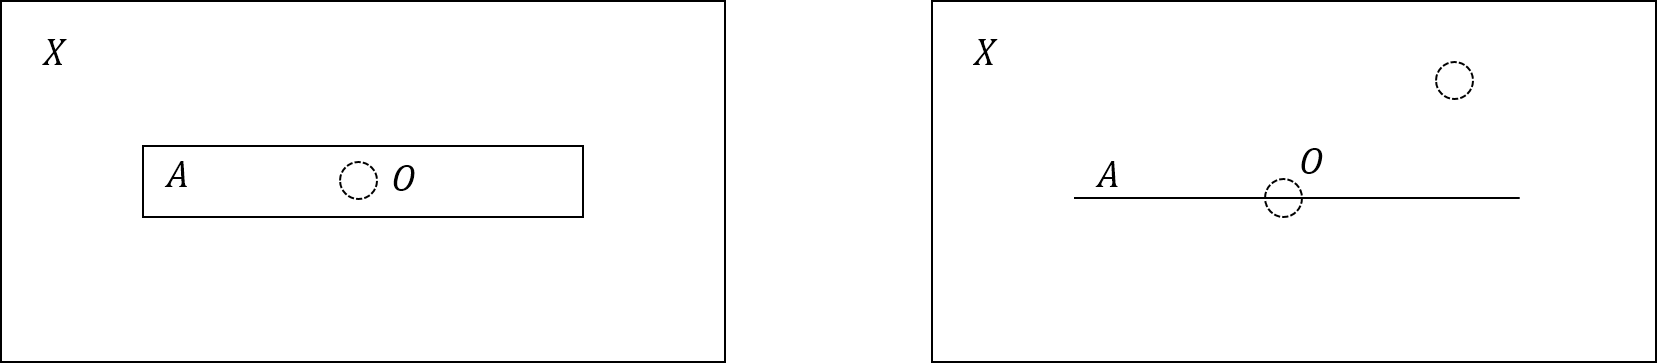
\includegraphics[width=\linewidth]{figure/集合内部非空.png}
\end{center}

再取反面,就可以得到

$$\mathring{A}=\emptyset \iff \forall \text{ 非空开子集 } O \in X, O\cap X-A\neq \emptyset $$

对应上图右边,无论怎么取开集,它都与补集有交.

后面证明Baire定理\ref{thm:baire:proof}时将要用到这种描述.

\subsection{闭包($\overline{A}$)}
在点集拓扑中,集合的闭包是指集合本身与集合的极限点构成的集合.比如一个圆,去掉内部一个点$x_0$,在集合中可以取一系列点,这些点逼近于$x_0$,则$x_0$属于闭包.一个开球的闭包还需要加上恰好在闭球的边界点.

给集合装备一种运算(实际上就是代数结构),假如集合中的元素在这种运算下生成的元素属于集合本身,那么说这个集合满足闭包性质.假如集合不闭合,那么包含这个集合的最小集合就是闭包.

对比这两种定义,可以看出它们本来是一回事,假如把点集拓扑中的“极限”当作一种运算,就是第二种定义.

\subsection{开集与闭集}
非常核心的概念.首先定义开集,闭集自然是对应的,或者取开集的补集.

\begin{enumerate}
	\item 距离空间中,所有点都是内点的集合是开集.
	\item 拓扑学中,所有开集构成拓扑,那么开集就是拓扑的元素.
\end{enumerate}

\subsection{紧性}
一开始有种直观理解是在任意两个点之间,都存在第三个点位于它们之间,假如这两个点恰好取在边界上,则不一定成立。比如平面上有一个洞,在这个洞的边界上取两个点,则它们的连线是在集合外。

现代数学中定义的紧性是基于有限子覆盖:如果一个拓扑空间$X$的所有开覆盖都有有限子覆盖。所谓“开覆盖”是指用开集族覆盖$X$,“子覆盖”就是开集族的子集覆盖$X$。

度量空间中的紧性是指:
\begin{enumerate}
\item 任意序列有收敛子序列,且子序列的极限点属于该集合。
\item 完备且完全有界。
\end{enumerate}

\subsection{稠密}
紧性是集合自身的性质,而稠密性还要涉及集合所处的空间。
\begin{definition}[稠密性]{}
给定拓扑空间$X$与一个子集$A$,如果对于$X$中任意一点$x$,它的邻域与$A$的交集非空。称$A$在$X$中稠密。等价于:

\begin{enumerate}
\item $\bar{A}=X$。
\end{enumerate}
\end{definition}

稠密性的直观理解是全空间中的任意一点都可以由子集中的点逼近。因此在逼近理论中非常有用。

一个简单的例子就是有理数在实数集的稠密性。因此任何一个实数都可以用有理数来逼近。但显然,有理数集自身不是紧的,因为一个有限数列的极限可以是无理数。

\subsection{可分性}
\begin{definition}[可分性]{}
一个距离空间如果有可数个稠密子集,则称为该空间可分。
\end{definition}

\section{集合的运算}
集合的差集$A-B$表示仅在$A$中,而不在$B$中的元素.

用$\Delta$表示对称差,$A\Delta B$表示属于并集,但不属于交集的元素,即仅在$A$或者仅在$B$中的元素.

$$A\Delta B=(A-B)\cup (B-A)$$

\paragraph*{分配律}

\begin{empheq}{align}
(A\cap B)\cup C&=(A\cup C)\cap (B\cup C) \\
(A\cup B)\cap C&=(A\cap C)\cup (B\cap C) \\
(A- B)\cap C&=(A\cap C)- (B\cap C)\\
(A- B)\cup C&=(A\cup C)- (B\cup C)\\
A-\cup B_k &=\cup(A-B_k)\\
A-\cap B_k &=\cap(A-B_k)
\end{empheq}

\paragraph*{de' morgan律}

\begin{empheq}{align}
	\overline{A\cup B}&=\overline{A}\cap \overline{B} \\
	\overline{A\cap B}&=\overline{A}\cup \overline{B} 
\end{empheq}

\section{集合论公理}
\subsection{六大基本公理}

\subsection{选择公理与Zorn引理}
两个定理是等价的,但Zorn引理方便使用一些.

\begin{definition}{选择公理}{sel}
设$(A_i)_{i\in I}$为某集合的一族子集,如果$I\neq \emptyset$,且$\forall i\in I,A_i\neq \emptyset$,则$\prod_{i\in I}A_i\neq\emptyset$.

乘积$\prod_{i\in I}A_i$(选择函数)是映射$f\colon I\rightarrow X$的集合,对$\forall i\in I,f(i)\in A_i$.

另一种表述:$X$非空,且每个元素非空,则存在选择函数.

这种描述中,$X$相当于$(A_i)_{i\in I}$.

\end{definition}

选择函数对每个$i$选择一个元素$f(i)\in A_i$.大致上相当于集合的外积、笛卡尔积.每个选择函数的定义域是相同的,而值域相当于笛卡尔集合中的一个元素.

注意选择公理本身并不是定理,而是人为加入的,仅由前六条公理无法得到选择公理的存在.

\begin{definition}{Zorn引理}{zorn}
设$X$为非空半序集,它的每个全序子集在$X$中均有上界,则$X$至少有一个极大元.
\end{definition}

